\documentclass[tikz]{standalone}
\usetikzlibrary{arrows,shapes,patterns}
\begin{document}
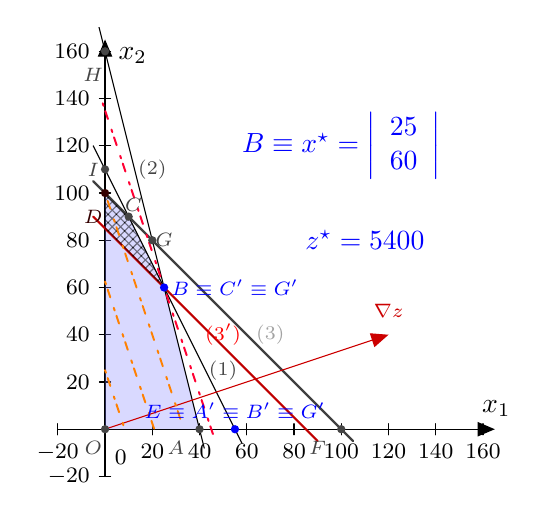
\begin{tikzpicture}[line cap=round,line join=round,>=triangle 45,x=0.03cm,y=0.03cm]
\definecolor{ffqqtt}{rgb}{1,0,0.2}
\definecolor{ccqqqq}{rgb}{0.8,0,0}
\definecolor{ttqqqq}{rgb}{0.2,0,0}
\definecolor{uuuuuu}{rgb}{0.27,0.27,0.27}
\definecolor{qqqqff}{rgb}{0,0,1}
\draw[->,color=black] (-20,0) -- (165,0);
\foreach \x in {-20,20,40,60,80,100,120,140,160}
\draw[shift={(\x,0)},color=black] (0pt,2pt) -- (0pt,-2pt) node[below] {\footnotesize $\x$};
\draw[color=black] (155.54,1.27) node [anchor=south west] {$x_1$};
\draw[->,color=black] (0,-20) -- (0,165);
\foreach \y in {-20,20,40,60,80,100,120,140,160}
\draw[shift={(0,\y)},color=black] (2pt,0pt) -- (-2pt,0pt) node[left] {\footnotesize $\y$};
\draw[color=black] (1.63,158.35) node [anchor=west] {$x_2$};
\draw[color=black] (0pt,-10pt) node[right] {\footnotesize $0$};
\clip(-20,-20) rectangle (180,170);

\fill[color=blue!50!white,opacity=0.3] (0,0)--(40,0)--(25,60)--(10,90)--(0,100)--cycle; %,pattern=north west lines
% vincolo 1
  \draw [domain=-5:58] plot(\x,{(--2200-40*\x)/20});
% vincolo 2
  \draw [domain=-5:42] plot(\x,{(--320-8*\x)/2});
% vincolo 3
  \draw [domain=-5:105,color=gray!50!black,line width=0.8pt] plot(\x,{(--100-1*\x)/1});
  \draw [domain=-5:90,color=red!75!black,line width=0.8pt] plot(\x,{(--85-1*\x)/1});
% gradiente
  \draw [->,color=ccqqqq] (0,0) -- (120,40);
% isoprofitto <= 5400
  \draw [line width=0.7pt,dash pattern=on 1pt off 2pt on 3pt off 4pt,color=ffqqtt,domain=-1:46] plot(\x,{(-5400--120*\x)/-40});
% nuova reg. amm.
  \fill[color=white!75,opacity=0.5,pattern=crosshatch] (0,85)--(25,60)--(10,90)--(0,100)--cycle; %,pattern=north west lines
\foreach \k in {1000, 2500, 4000}
  \draw [line width=0.7pt,dash pattern=on 1pt off 2pt on 3pt off 4pt,color=orange,domain=0:\k/120] plot(\x,{(-\k--120*\x)/-40});

\begin{scriptsize}
% punto O
  \fill [color=uuuuuu] (0,0) circle (1.5pt);
  \draw[color=uuuuuu] (-5,-8) node {$O$};
% punto E
  \fill [color=qqqqff] (55,0) circle (1.5pt);
  \draw[color=qqqqff] (55,8) node {$E \equiv A^\prime \equiv B^\prime \equiv G^\prime$};
% punto I
  \fill [color=uuuuuu] (0,110) circle (1.5pt);
  \draw[color=uuuuuu] (-5,110) node {$I$};
% punto A
  \fill [color=uuuuuu] (40,0) circle (1.5pt);
  \draw[color=uuuuuu] (30,-8) node {$A$};
% punto H
  \fill [color=uuuuuu] (0,160) circle (1.5pt);
  \draw[color=uuuuuu] (-5,150) node {$H$};
% punto B
  \fill [color=qqqqff] (25,60) circle (1.5pt);
  \draw[color=qqqqff] (55,60) node {$B \equiv C^\prime \equiv G^\prime$};
  \fill [color=uuuuuu] (100,0) circle (1.5pt);
  \draw[color=uuuuuu] (90,-8) node {$F$};
  \fill [color=ttqqqq] (0,100) circle (1.5pt);
  \draw[color=ttqqqq] (-5,90) node {$D$};
  \fill [color=uuuuuu] (10,90) circle (1.5pt);
  \draw[color=uuuuuu] (12,95) node {$C$};
  \fill [color=uuuuuu] (20,80) circle (1.5pt);
  \draw[color=uuuuuu] (25,80) node {$G$};

  \draw[color=ccqqqq] (120,50) node {$\nabla z$};
  
  \draw[color=uuuuuu] (50, 25) node {$(1)$};
  \draw[color=uuuuuu] (20,110) node {$(2)$};
  \draw[color=uuuuuu!50] (70, 40) node {$(3)$};
  \draw[color=red] (50, 40) node {$(3^\prime)$};
\end{scriptsize}
  \draw[color=qqqqff] (100,120) node {$B \equiv x^{\star} = \left|\begin{array}{c}25\\60\end{array}\right|$};
  \draw[color=qqqqff] (110, 80) node {$		z^{\star} = 5400$};
\end{tikzpicture}
\end{document}